\documentclass[11pt]{article}

\usepackage{amsmath, amssymb}
\usepackage{geometry}
\usepackage{graphicx}
\usepackage{booktabs}

\geometry{margin=1in}

\title{Finite Difference Methods for the Black--Scholes Equation}
\author{Robin Basso}
\date{\today}

\begin{document}

\maketitle

\section{Introduction}

The Black--Scholes equation is a fundamental partial differential equation (PDE) in quantitative finance used to price European options. This project implements and analyzes several finite difference schemes to solve the PDE numerically.

The objectives are:
\begin{itemize}
    \item Implement explicit and Crank--Nicolson schemes
    \item Validate numerical solutions against the analytical formula
    \item Study spatial and temporal convergence
    \item Analyze stability and the effect of payoff regularity
\end{itemize}

\section{Black--Scholes Model}

The Black--Scholes PDE is given by:
\begin{equation}
\frac{\partial V}{\partial t}
+ \frac{1}{2} \sigma^2 S^2 \frac{\partial^2 V}{\partial S^2}
+ r S \frac{\partial V}{\partial S}
- r V = 0
\end{equation}

where:
\begin{itemize}
    \item $S$ is the asset price
    \item $t$ is time
    \item $\sigma$ is volatility
    \item $r$ is the risk-free rate
\end{itemize}

\subsection{Terminal Condition}

For a European call option:
\begin{equation}
V(S, T) = \max(S - K, 0)
\end{equation}

\subsection{Boundary Conditions}

\begin{align}
V(0, t) &= 0 \\
V(S_{\max}, t) &\approx S_{\max} - K e^{-r(T-t)}
\end{align}

\section{Discretization}

We discretize:
\begin{itemize}
    \item Space: $S_i = i \Delta S$
    \item Time: $t^n = n \Delta t$
\end{itemize}

\subsection{Finite Differences}

\begin{align}
\frac{\partial V}{\partial t} &\approx \frac{V_i^{n+1} - V_i^n}{\Delta t} \\
\frac{\partial V}{\partial S} &\approx \frac{V_{i+1}^n - V_{i-1}^n}{2\Delta S} \\
\frac{\partial^2 V}{\partial S^2} &\approx \frac{V_{i+1}^n - 2V_i^n + V_{i-1}^n}{\Delta S^2}
\end{align}

\section{Explicit Scheme}

Substituting finite differences into the PDE gives:

\begin{equation}
V_i^n = a_i V_{i-1}^{n+1} + b_i V_i^{n+1} + c_i V_{i+1}^{n+1}
\end{equation}

with:
\begin{align}
a_i &= \frac{1}{2} \Delta t (\sigma^2 i^2 - r i) \\
b_i &= 1 - \Delta t (\sigma^2 i^2 + r) \\
c_i &= \frac{1}{2} \Delta t (\sigma^2 i^2 + r i)
\end{align}

\subsection{Stability}

The explicit scheme is conditionally stable and requires:
\begin{equation}
\Delta t \lesssim \frac{1}{\sigma^2 M^2}
\end{equation}

\section{Crank--Nicolson Scheme}

The Crank--Nicolson method is obtained by averaging between time levels $n$ and $n+1$.

This leads to a linear system:
\begin{equation}
A V^n = B V^{n+1}
\end{equation}

where $A$ and $B$ are tridiagonal matrices.

\subsection{Properties}

\begin{itemize}
    \item Second-order accurate in time and space
    \item Unconditionally stable
\end{itemize}

\section{Rannacher Smoothing}

The payoff function is not smooth at $S = K$, which degrades convergence.

To address this, we use:
\begin{itemize}
    \item First few time steps: implicit Euler
    \item Remaining steps: Crank--Nicolson
\end{itemize}

This improves numerical stability and convergence behavior.

\section{Convergence Analysis}

\subsection{Spatial Convergence}

Both schemes exhibit:
\begin{equation}
\text{Error} = \mathcal{O}(\Delta S^2)
\end{equation}

\subsection{Time Convergence}

\begin{itemize}
    \item Explicit: $\mathcal{O}(\Delta t)$
    \item Crank--Nicolson: $\mathcal{O}(\Delta t^2)$ (theoretical)
\end{itemize}

However, in practice:

\begin{itemize}
    \item Time convergence is difficult to observe for the explicit scheme due to stability constraints
    \item Crank--Nicolson convergence is degraded by the non-smooth payoff
\end{itemize}

\subsection{Effect of Payoff Regularity}

The payoff:
\begin{equation}
V(S,T) = \max(S-K,0)
\end{equation}

is not differentiable at $S=K$, leading to:
\begin{itemize}
    \item Reduced convergence order
    \item Dominance of spatial error
\end{itemize}

\section{Numerical Results}

\subsection{Validation}

\includegraphics[width=0.8\textwidth]{comparison.png}

\subsection{Spatial Convergence}

\includegraphics[width=0.8\textwidth]{convergence.png}

\subsection{Time Convergence (Rannacher)}

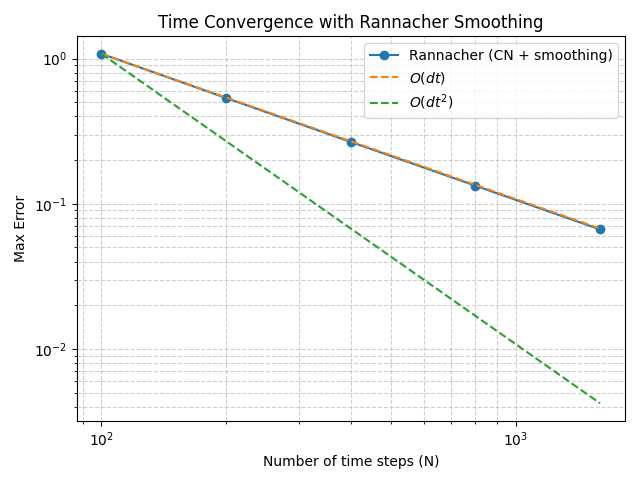
\includegraphics[width=0.8\textwidth]{tests/time_convergence_rannacher.png}

\section{Conclusion}

This study highlights several important aspects of numerical PDE solving:

\begin{itemize}
    \item Finite difference methods accurately reproduce Black--Scholes prices
    \item Stability constraints strongly affect explicit schemes
    \item Spatial convergence is robust and second-order
    \item Time convergence is limited by payoff regularity
    \item Rannacher smoothing improves practical convergence behavior
\end{itemize}

These results illustrate key trade-offs between stability, accuracy, and computational cost in numerical option pricing.

\end{document}